\section{Versuchsaufbau und Messgeräte}
\begin{figure}[htbp]  
     \usetikzlibrary{shapes,arrows}
\tikzstyle{block} = [draw, fill=blue!20, rectangle, 
    minimum height=1em, minimum width=2em]
\tikzstyle{circle} = [draw, fill=blue!20, ellipse, 
    minimum height=1.5em, minimum width=1.5em]
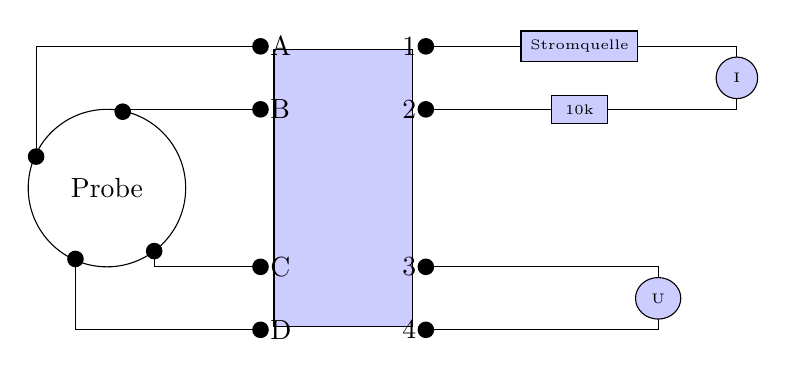
\begin{tikzpicture}
 \coordinate (L) at (-5,0);
\coordinate (R1) at (2,-1.4);
\coordinate (R2) at (3,1.4);
\coordinate (M1) at (1, 1.0);
\coordinate (M2) at (1, 1.8);


 \coordinate (A1) at (-5.9,0.4);
\coordinate (B1) at (-4.8,0.97);
\coordinate (C1) at (-4.4,-0.8);
\coordinate (D1) at (-5.4,-0.9);

\coordinate (A2) at (-3.05,1.8);
\coordinate (B2) at (-3.05,1.0);
\coordinate (C2) at (-3.05,-1.0);
\coordinate (D2) at (-3.05,-1.8);

\coordinate (A3) at (-0.95,1.8);
\coordinate (B3) at (-0.95,1.0);
\coordinate (C3) at (-0.95,-1.0);
\coordinate (D3) at (-0.95,-1.8);
\draw (L) circle [radius=1];
\node (probe) at (L) {Probe};

\fill[black] (A1) circle (3pt);
\fill[black] (B1) circle (3pt);
\fill[black] (C1) circle (3pt);
\fill[black] (D1) circle (3pt);

\node[block, minimum height=10em, minimum width=5em] at (-2,0) {};
\fill[black] (A2) circle (3pt);
\fill[black] (B2) circle (3pt);
\fill[black] (C2) circle (3pt);
\fill[black] (D2) circle (3pt);
\draw (A1) |- (A2);
\draw (B1) |- (B2);
\draw (C1) |- (C2);
\draw (D1) |- (D2);
\fill[black] (A3) circle (3pt);
\fill[black] (B3) circle (3pt);
\fill[black] (C3) circle (3pt);
\fill[black] (D3) circle (3pt);
\draw (A2) node[right] {A};
\draw (B2) node[right] {B};
\draw (C2) node[right] {C};
\draw (D2) node[right] {D};
\draw (A3) node[left] {1};
\draw (B3) node[left] {2};
\draw (C3) node[left] {3};
\draw (D3) node[left] {4};

\draw (D3) -| (R1);
\draw (C3) -| (R1);
\node[circle] at (R1) {\tiny U};

\draw (B3) -- (M1);
\draw (M1) -| (R2);
\draw (A3) -- (M2);
\draw (M2) -| (R2);
\node[block] at (M1) {\tiny 10k};
\node[circle] at (R2) {\tiny I};
\node[block] at (M2) {\tiny Stromquelle};
\end{tikzpicture}
  \caption{Schematischer Versuchsaufbau zu Messung der zurückgestreuten Helium-Ionen, $\theta=171^\circ$}
  \label{aufbau}
\end{figure}

In \ref{aufbau} ist der prinzipielle Versuchsaufbau mit Target und Detektor dargestellt. Das Target befindet sich dabei in einer Vakuumkammer, welche zum Wechseln des Targets vom Strahlsystem abgekoppelt werden kann. Wichtig dabei ist die vorherige Schließung der vorhandenen  Shutter, um den Strahl nicht mehr bis zum Target vordringen zu lassen. Zur Entlüftung der Kammer wird eine Turbopumpe verwendet, welche über direkt am Versuchsaufbau steuerbare Ventile mit der Kammer verbindbar bzw. von der Kammer abtrennbar ist. Über sie wird jedes mal nach Einsetzen eines neuen Targets der Druck in der Kammer auf $p \approx 10^{-6} mbar$ abgesenkt. Nach Einsetzen der Probe ist weiterhin auf die Erdung des Probenträgers zu achten, da sonst statische Aufladungen entstehen können. 
